\documentclass{beamer}

% Pri pouziti XeLaTeX pouzij unicode fonty
\usepackage{fontspec}
\usepackage{xunicode}
\usepackage{xltxtra}
\usepackage{multirow}

\usepackage{graphicx}			% Balíček 'graphicx' pro vkládání obrázků
%\usepackage{ucs}
%\usepackage{palatino}
%\inputencoding{utf8}
\usepackage[czech]{babel}
\usepackage{amsmath}
\usepackage{amsfonts}

\usepackage{pgfpages}
\usetheme{Madrid}
%\usecolortheme[named=OliveGreen]{structure}

\title{Zigbee kanálový analyzátor}
\author[Potfay, Slinták]{Attila Potfay\\Vlastimil Slinták}
\institute[MSSY]{%
MSSY -- Bezdrátové senzorové sítě
}
\date{2.\,května\,2013}

\begin{document}
	% ---------------------------------------------------------------------
	% Uvodni stranka
	\frame{\titlepage}

	% ---------------------------------------------------------------------
	\begin{frame}
	\frametitle{Firmware pro kanálový analyzátor}
	\begin{itemize}
	\item Firmware pro vysílač
	\item Firmware pro přijímač
	\item Použitý ZigBee kanál -- 17
	\end{itemize}
	\end{frame}

	% ---------------------------------------------------------------------
	\begin{frame}
	\frametitle{Spektrum v okolí učebny}
	\begin{figure}[!ht]
	\centering%
	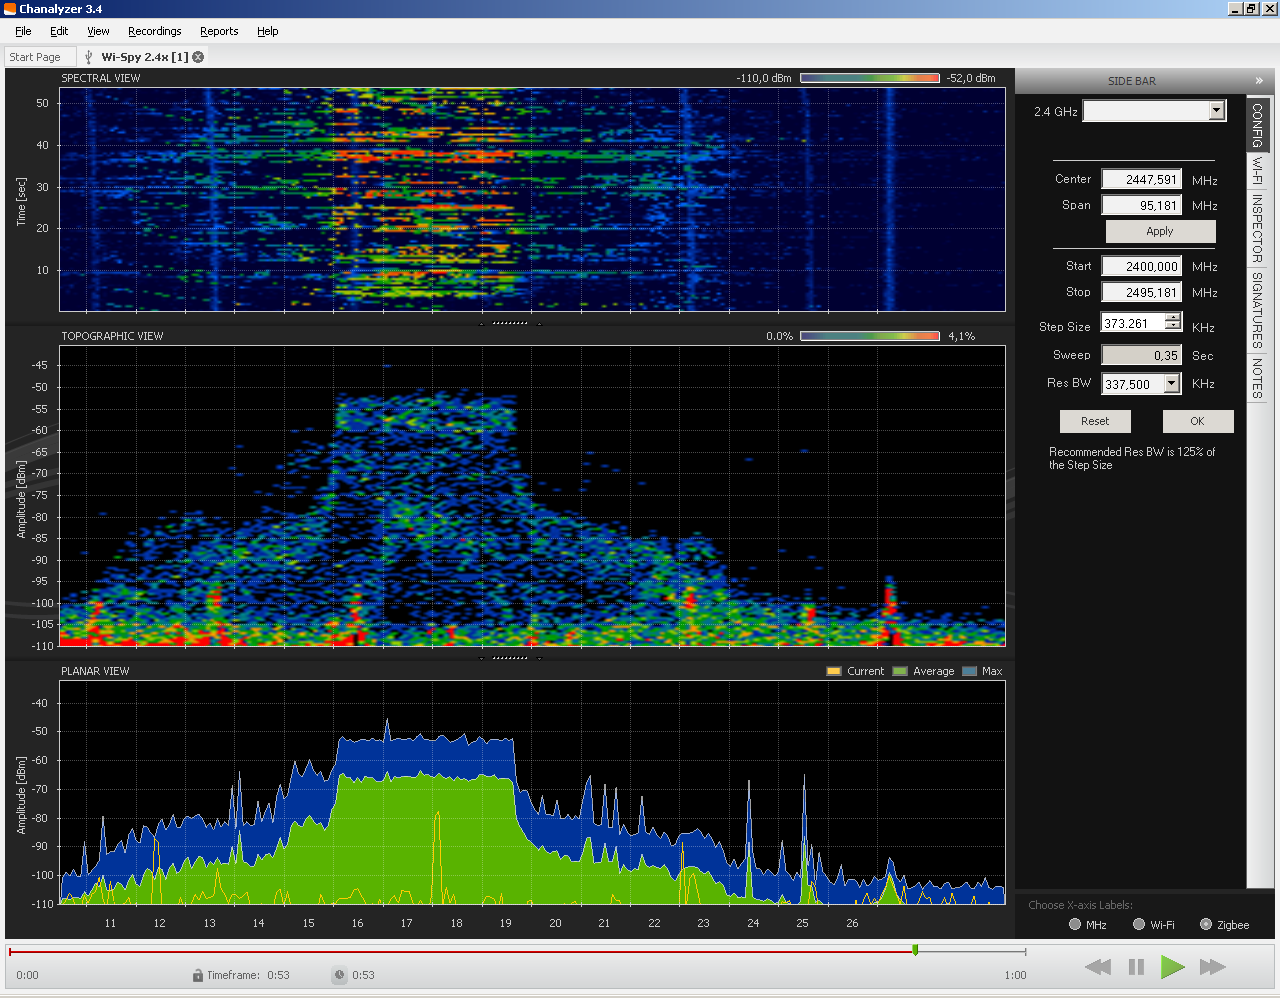
\includegraphics[scale=0.2, keepaspectratio]{spektrum}%
	\caption{Spektrum změřené programem Chanalyzer (ZigBee kanály)}
	\end{figure}
	\end{frame}

	\begin{frame}
	\frametitle{Spektrum v okolí učebny}
	\begin{figure}[!ht]
	\centering%
	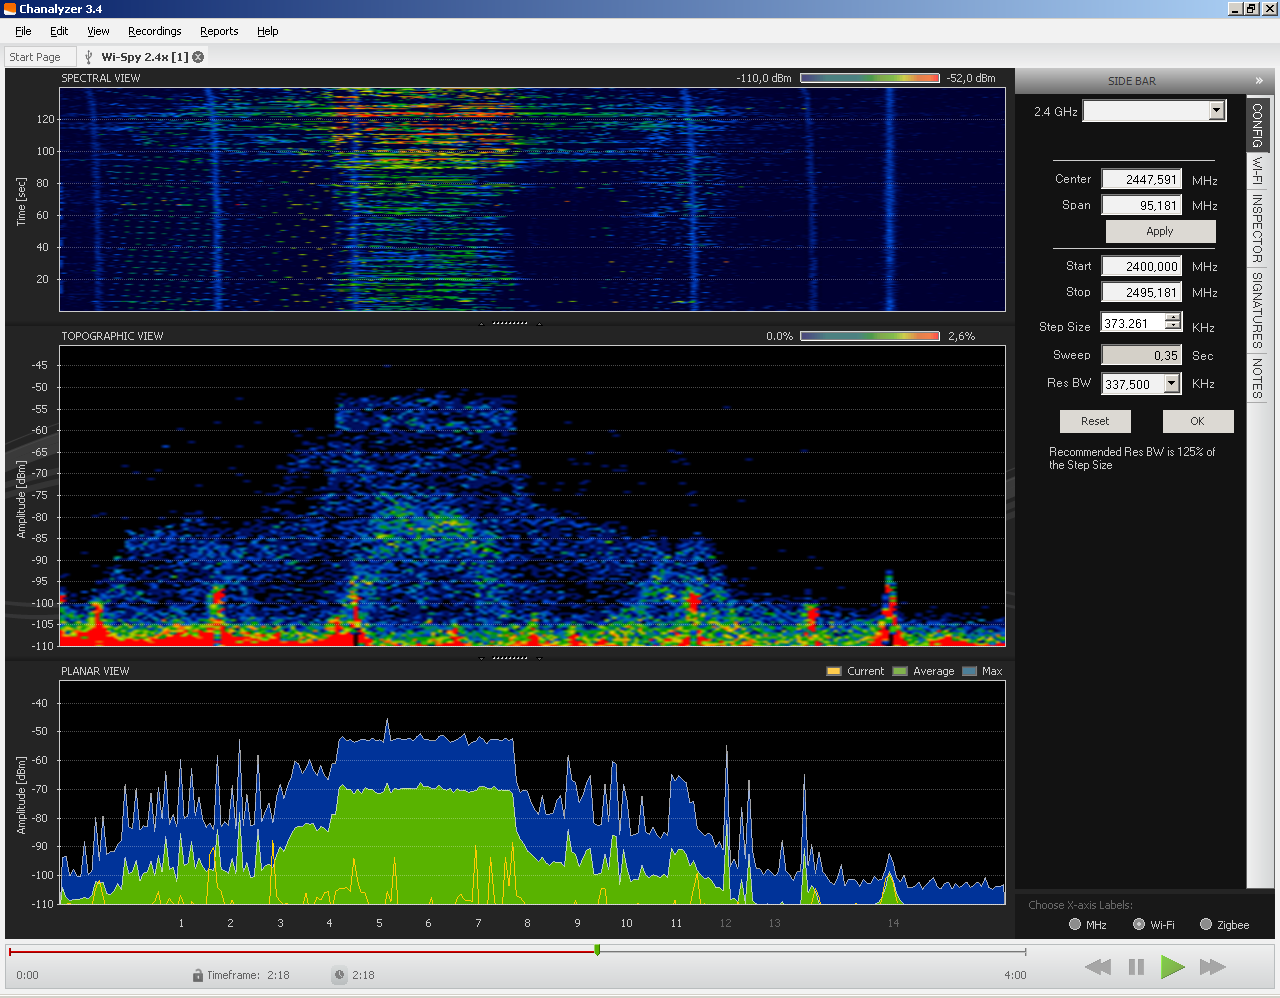
\includegraphics[scale=0.2, keepaspectratio]{spektrum2}%
	\caption{Spektrum změřené programem Chanalyzer (Wifi kanály)}
	\end{figure}
	\end{frame}

	\begin{frame}
	\frametitle{Kde probíhalo měření}
	\begin{figure}[!ht]
	\centering%
	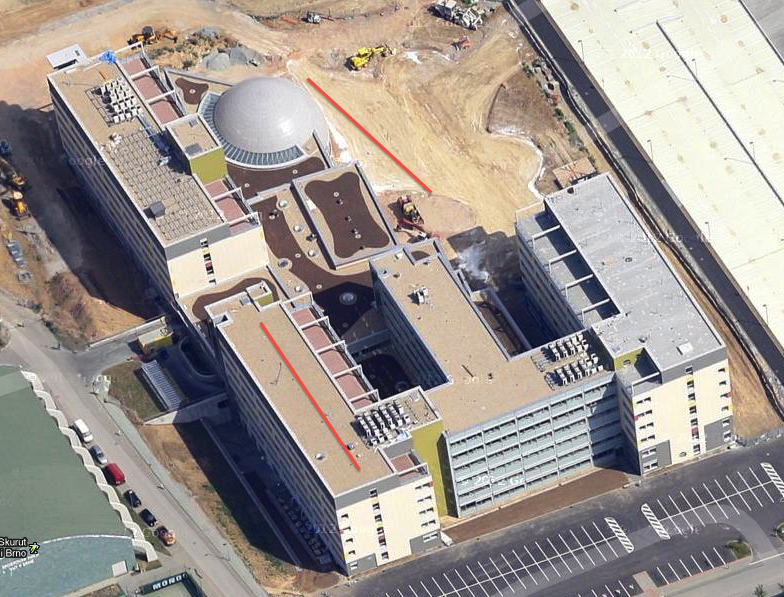
\includegraphics[scale=0.3, keepaspectratio]{mapa}%
	\caption{Letecký snímek budovy FEKT, zdroj Google Maps}
	\end{figure}
	\end{frame}

	% ---------------------------------------------------------------------
	\begin{frame}
	\frametitle{Zjištění komunikačního dosahu}
	\begin{table}[ht!]
	\centering
	\begin{tabular}{|c|c|c|c|} \hline
	Místo měření& Výkon & Vzdálenost & PDR \\
	& [dBm] & [m] & [\%] \\ \hline \hline
	\multirow{2}{*}{Uvnitř} & 3 & 33 & 88 \\
	& -17 & 11 & 75 \\ \hline

	\multirow{2}{*}{Venku} & 3 & 42-43 & 83 \\
	& -17 & 13 & 78 \\ \hline
	\end{tabular}
	\end{table}
	\end{frame}

	\begin{frame}
	\frametitle{Měření závislosti vzdálenosti vysílače od koordinátora}
	\framesubtitle{Měření uvnitř budovy}
	\begin{figure}[!ht]
	\centering%
	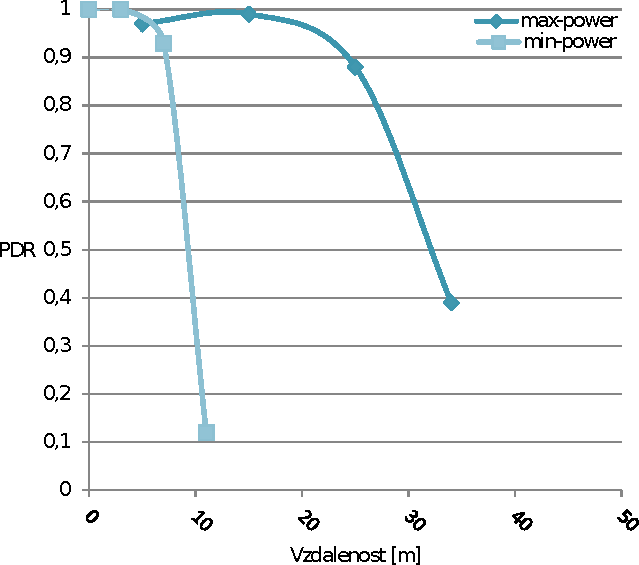
\includegraphics[scale=0.7, keepaspectratio]{2-pdr}%
	\caption{Packet Delivery Ratio, uvnitř budovy}
	\end{figure}
	\end{frame}

	\begin{frame}
	\frametitle{Měření závislosti vzdálenosti vysílače od koordinátora}
	\framesubtitle{Měření uvnitř budovy}
	\begin{figure}[!ht]
	\centering%
	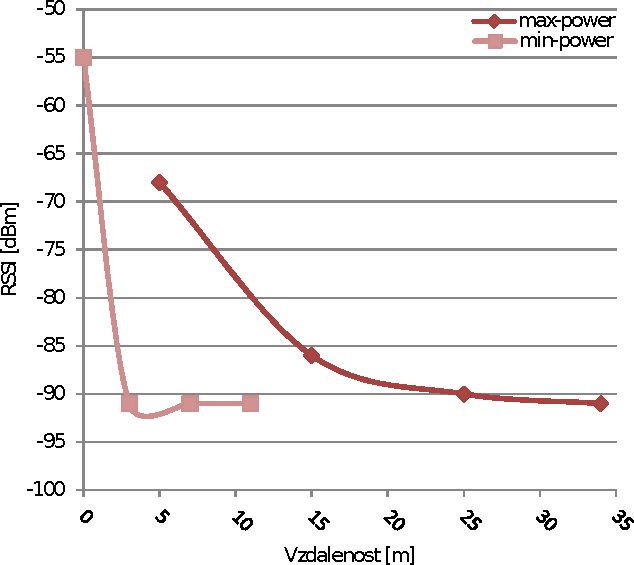
\includegraphics[scale=0.7, keepaspectratio]{2-rssi}%
	\caption{RSSI, uvnitř budovy}
	\end{figure}
	\end{frame}

	\begin{frame}
	\frametitle{Měření závislosti vzdálenosti vysílače od koordinátora}
	\framesubtitle{Měření uvnitř budovy}
	\begin{figure}[!ht]
	\centering%
	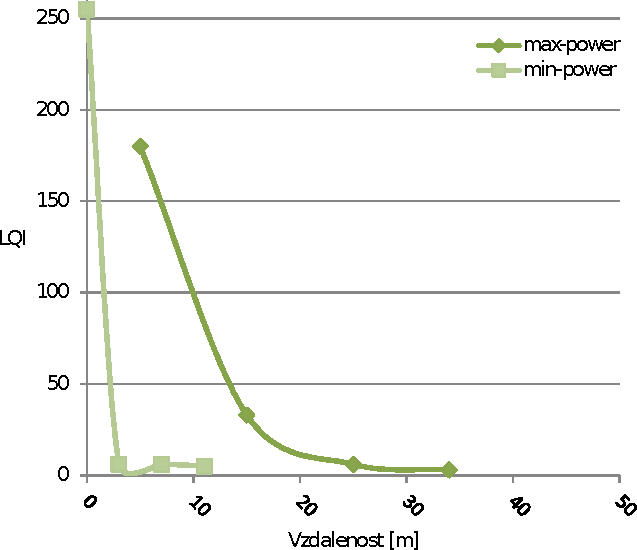
\includegraphics[scale=0.7, keepaspectratio]{2-lqi}%
	\caption{LQI, uvnitř budovy}
	\end{figure}
	\end{frame}

	\begin{frame}
	\frametitle{Měření závislosti vzdálenosti vysílače od koordinátora}
	\framesubtitle{Měření před budovou}
	\begin{figure}[!ht]
	\centering%
	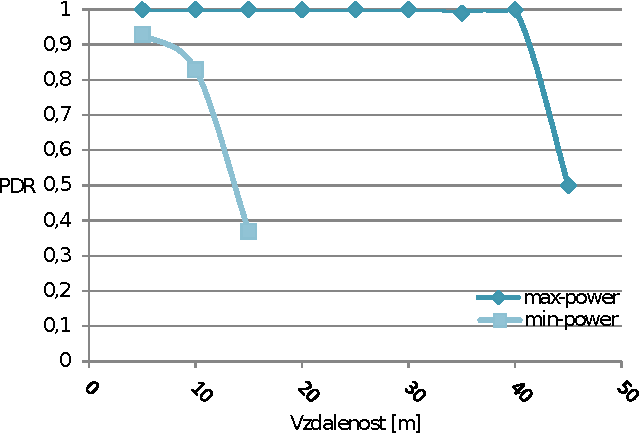
\includegraphics[scale=0.7, keepaspectratio]{2-pdr-venku}%
	\caption{Packet Delivery Ratio, před budovou}
	\end{figure}
	\end{frame}

	\begin{frame}
	\frametitle{Měření závislosti vzdálenosti vysílače od koordinátora}
	\framesubtitle{Měření před budovou}
	\begin{figure}[!ht]
	\centering%
	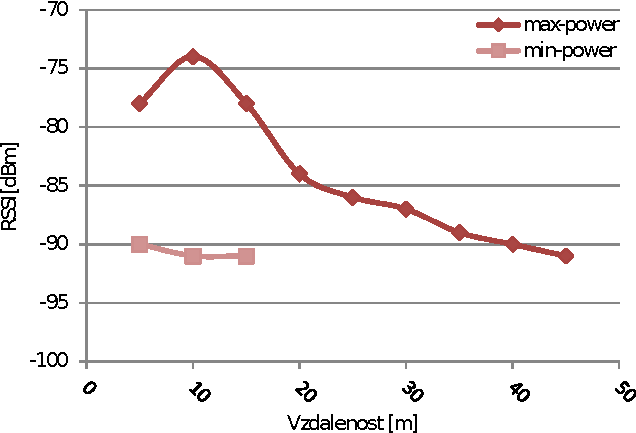
\includegraphics[scale=0.7, keepaspectratio]{2-rssi-venku}%
	\caption{RSSI, před budovou}
	\end{figure}
	\end{frame}

	\begin{frame}
	\frametitle{Měření závislosti vzdálenosti vysílače od koordinátora}
	\framesubtitle{Měření před budovou}
	\begin{figure}[!ht]
	\centering%
	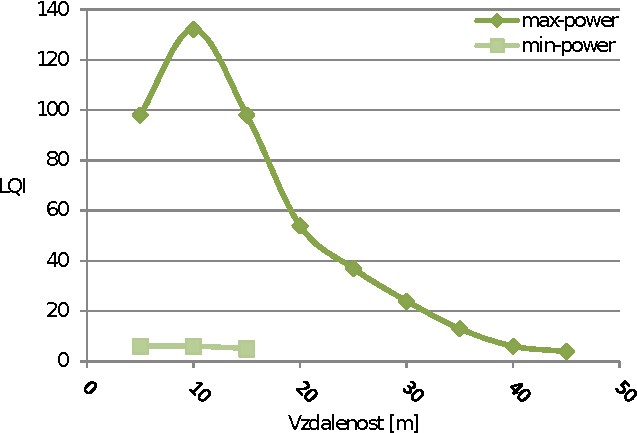
\includegraphics[scale=0.7, keepaspectratio]{2-lqi-venku}%
	\caption{LQI, před budovou}
	\end{figure}
	\end{frame}

	\begin{frame}
	\frametitle{Statistické měření kvalitativních parametrů}
	\begin{figure}[!ht]
	\centering%
	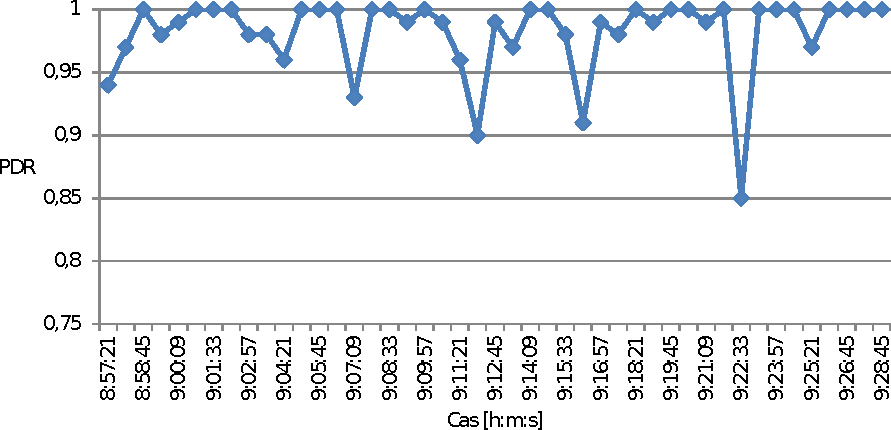
\includegraphics[scale=0.7, keepaspectratio]{3-pdr}%
	\caption{Packet Delivery Ratio, uvnitř budovy}
	\end{figure}
	\end{frame}

	\begin{frame}
	\frametitle{Statistické měření kvalitativních parametrů}
	\begin{figure}[!ht]
	\centering%
	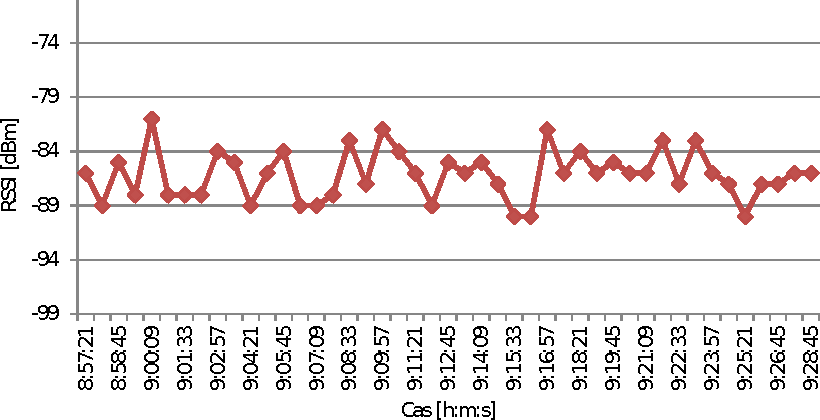
\includegraphics[scale=0.7, keepaspectratio]{3-rssi}%
	\caption{RSSI, uvnitř budovy}
	\end{figure}
	\end{frame}

	\begin{frame}
	\frametitle{Statistické měření kvalitativních parametrů}
	\begin{figure}[!ht]
	\centering%
	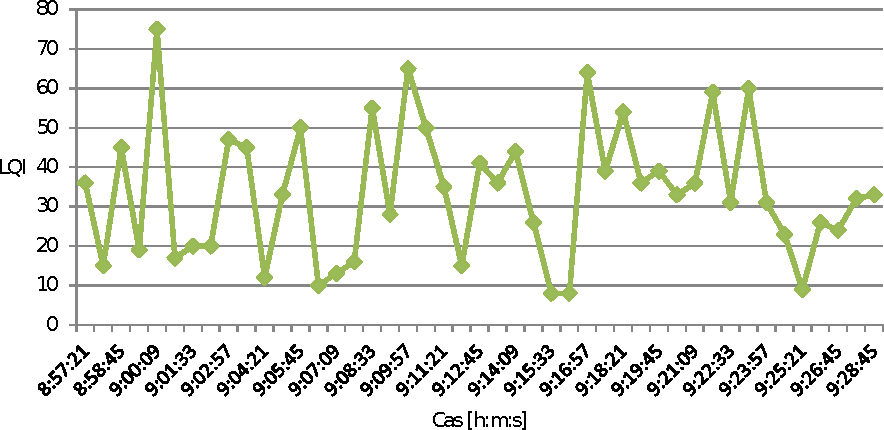
\includegraphics[scale=0.7, keepaspectratio]{3-lqi}%
	\caption{LQI, uvnitř budovy}
	\end{figure}
	\end{frame}


\end{document}
